\chapter{System Design}

\begin{figure}[!htbp]
	\centering
	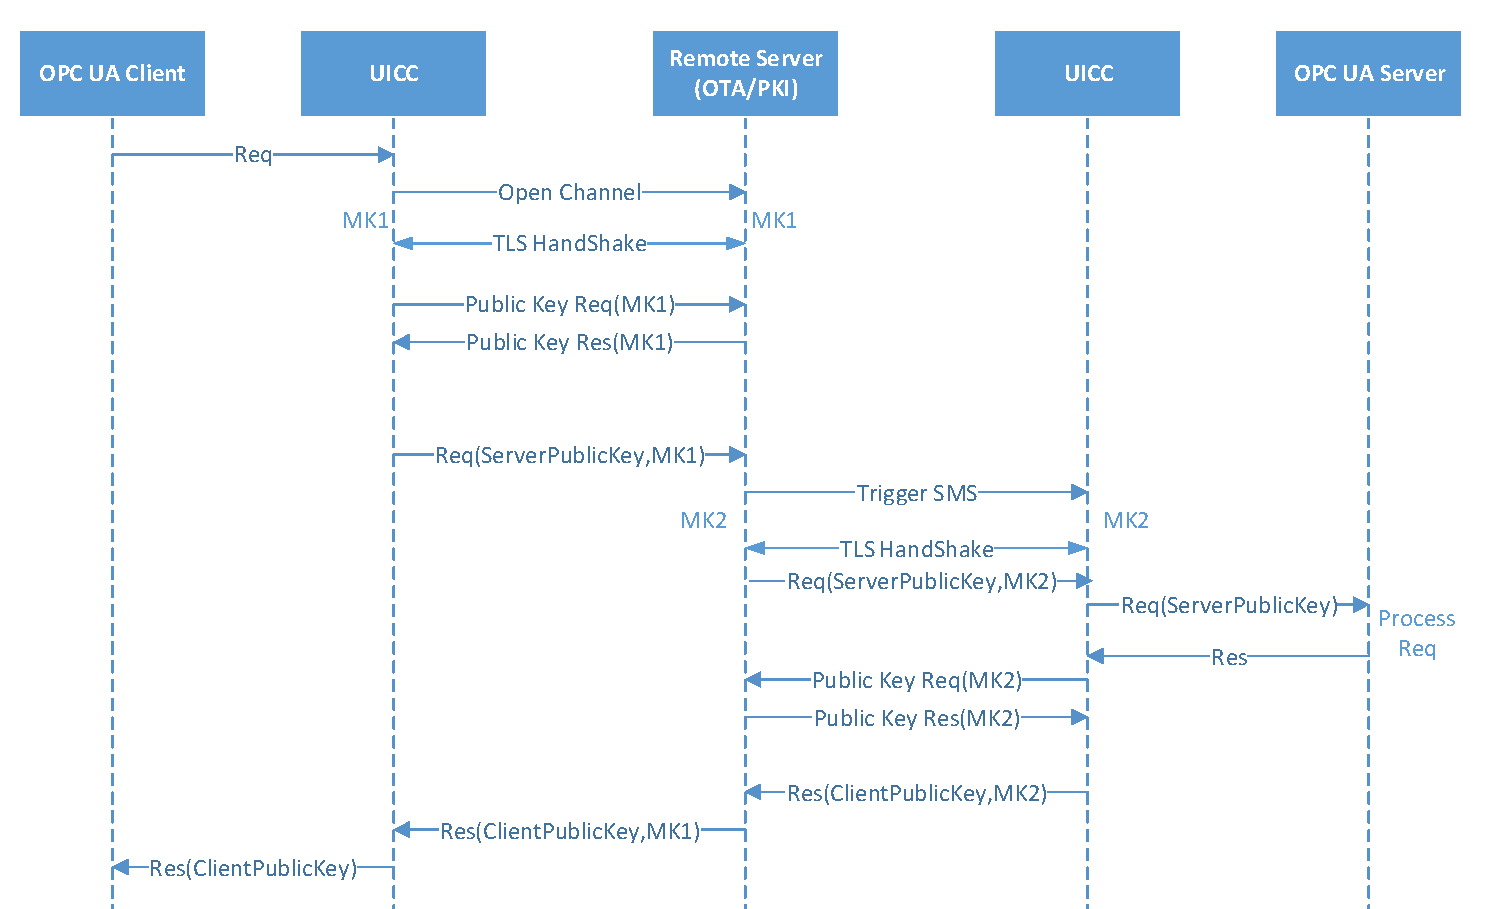
\includegraphics[width=1\textwidth]{whole-structure}
		\caption{Message Exchange}
	\label{fig:whole-structure}
\end{figure}
In this chapter, I will present the crucial information about how I designed and programmed my system. To be more specifically, I am going to describe the design of my UICC Applet, Android  Application as well as  Smart  Home Web Server.

As described in previous chapters, my demonstration system consists of three main parts, namely the on card integrated communication stack, Android application and Smart Home web service. Figure~\ref{fig:whole-structure} illustrates the request and corresponding response message exchange process that occurs in the demonstration system. In my case, OTA is also integrated with a \emph{public key infrastructure},  in order to perform secure peer identification and messaging. Therefor this OTA is also referred as remote administrator sever.


\section{UICC Applet}
\subsection{Overview}
The whole message exchange process consists of following phases:
\begin{itemize}
\item \emph{Open Channel Phase} Whenever a secure housing device attempts to contact with the other, a communication session between Remote Server and this device must be created firstly.
\item \emph{TSL Handshake with Remote Server} After a successful creation of communication channel, a mutual peer identification through TLS handshake between Remote server and aforementioned homing device will be performed.
\item \emph{Require target's public key} When Remote Server identify the connected communication partner, it will grant him the expected target's public key. 
\item \emph{secure messaging} Message sender will in this phase encrypt the message with target's public key and send this encrypted message through Remote Server to message receiver. 
\end{itemize}
\subsection {Work Flow}

The components involved in this scenario are:
 \begin{itemize}
  \item CommunicationStack applet and associated Security Domain from Globalplatform (APSD  for short)
  \item OTA-PKI server which is also known as Remote Administration Server (RAS for short)
\end{itemize}

The communication between CommunicationStack and Remote Administration Server involves following  steps:

 \begin{itemize}
  \item Open Communication Channel and Create Communication Session
  \item Secure Message Exchange
  \item Close Communication Session
\end{itemize}
\subsubsection{Communication Session Creation and Message Exchange}
This process could be either initiated by Remote Administration Server by sending target applet a trigger SMS or be sponsored by applet itself. In both cases, \emph{CommunicationStack} applet sends the first \emph{OpenChannel Request} message. During the PSK TLS Handshake phase, APSD and remote server will agree on the to be used cipher suit and authenticate each other. After a successful PSK TLS Handshake, remote server will then grant authenticated user the public key of his target applet and forward his following Http message, which encapsulates APDU command or response strings as body. The Http header is in compliance with GlobalPlatform standards and shown in following.


\begin{figure}[!htbp]
	\centering
	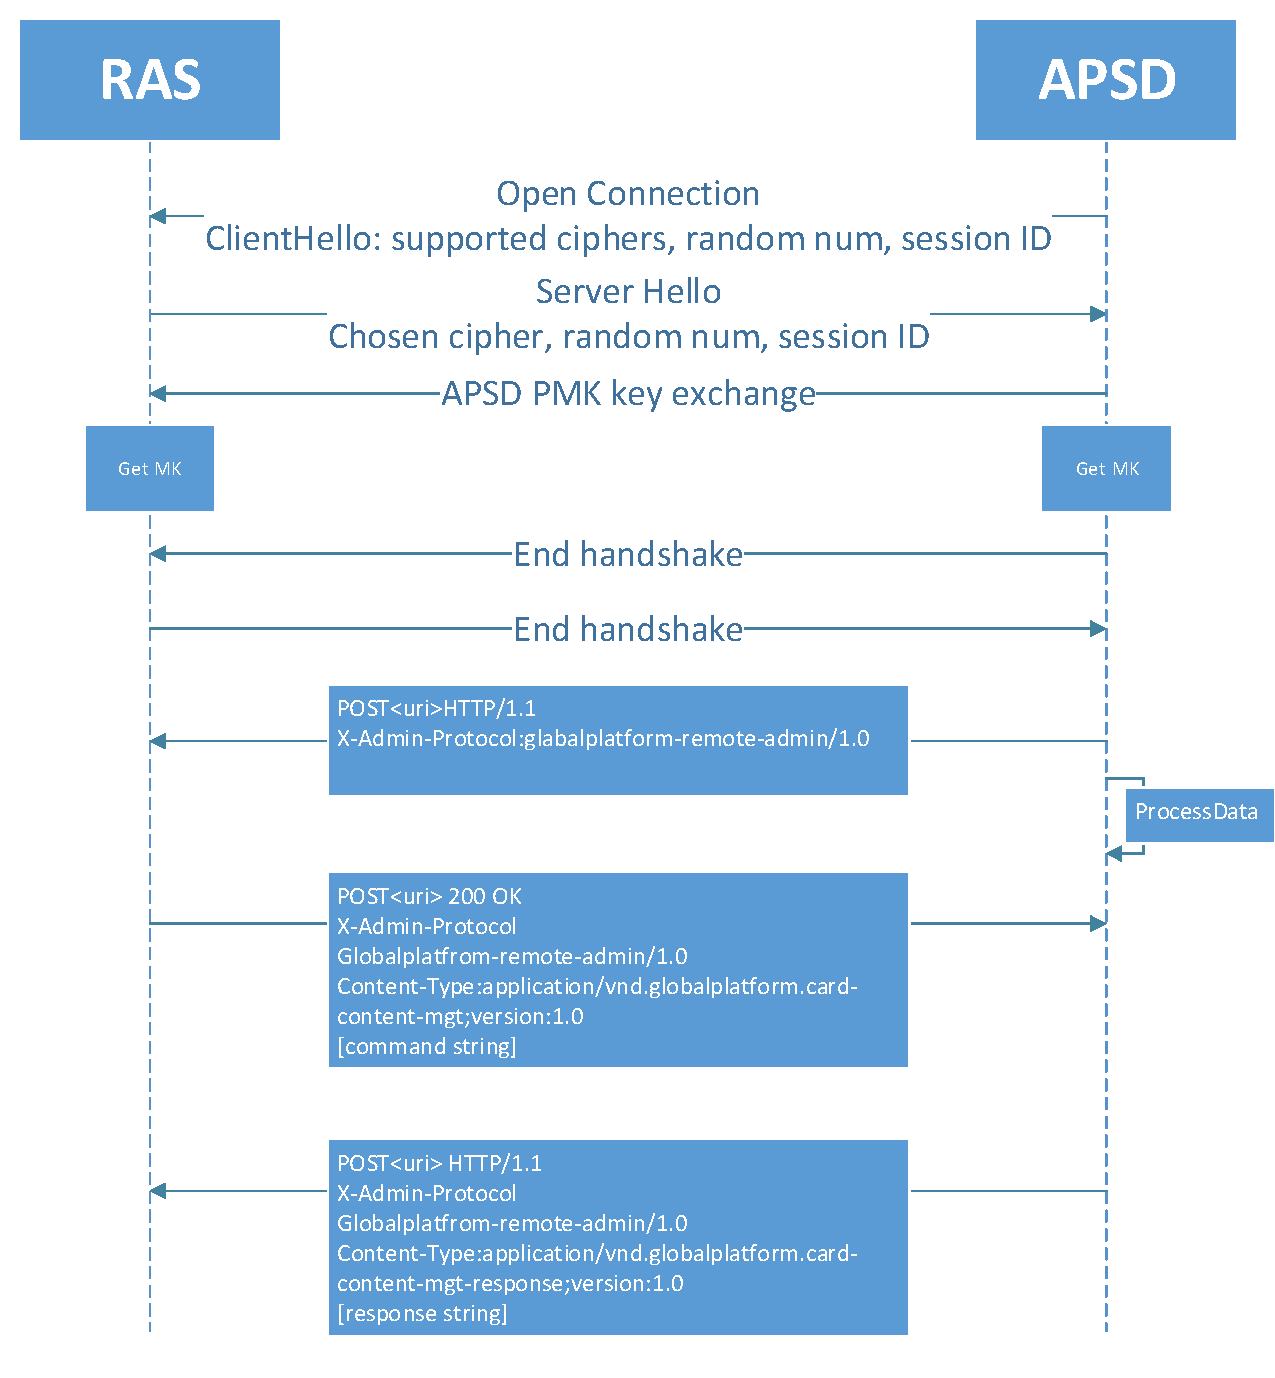
\includegraphics[width=1\textwidth]{communication-flow}
		\caption{Handshake and message exchange between SD and Remote Server}
	\label{fig:communication-flow}
\end{figure}

\subsubsection{Http Header Format} \label{secHTTPHeader}
The Http message sent from remote sever to targeted applet obeys following schema\cite{gp}:
\begin{Verbatim}[fontsize=\relsize{-1}, frame=lines,framesep=4mm, label=\fbox{\small\emph{Http Request Schema}}]
HTTP/1.1 200 OK [or HTTP/1.1 204 No Content CRLF]
X-Admin-Protocol: globalplatform-remote-admin/1.0 CRLF
[X-Admin-Next-URI:  <next-URI> CRLF]
[Content-Type: application/vnd.globalplatform.card-content-mgt
-response;version=1.0 CRLF]
[X-Admin-Targeted-Application: <security-domain-AID> CRLF]
[Content-Length: xxxx CRLF] or [Transfer-Encoding: chunked CRLF]
CRLF
[body]
\end{Verbatim}
The field \emph{security-domain-AID} will be filled with the AID of targeted applet.


The Http response message sent from applet to remote server uses following schema\cite{gp}:
\begin{Verbatim}[fontsize=\relsize{-1}, frame=lines,framesep=4mm, label=\fbox{\small\emph{Http Response Schema}}]
POST<URI>HTTP/1.1 CRLF
Host: <Administration Host> CRLF
X-Admin-Protocol: globalplatform-remote-admin/1.0 CRLF
X-Admin-From: <Agent ID> CRLF
[Content-Type: application/vnd.globalplatform.card-content-mgt
-response;version=1.0 CRLF]
[Content-Length: xxxx CRLF] or [Transfer-Encoding: chunked CRLF]
[X-Admin-Script-Status: <script-status> CRLF]
[X-Admin-Resume: true]
CRLF
[body]
\end{Verbatim}

The filed \emph{X-Admin-Script-Status} could contain following values:
 \begin{itemize}
  \item \emph{ok}, which means that the previous message is successfully received by applet.
  \item \emph{unknown-application}, which stands for the error, that the targeted applet for previous message can not be found.
\item \emph{not-a-security-domain}, this errors occurs when targeted applet is not a Security Domain.
\item \emph{security-error}, as its name indicates, this values is returned if the security of previous message  can not be checked.
\end{itemize}

\subsubsection{Close Communication Session}
Whenever the communication channel is about to be closed, either because of session security issue, or due to successful finish of communication, remote server will send target applet Http message using following parameters:
 \begin{itemize}
  \item No \emph{X-Admin-Next-URI} field is present in this Http message and message body is empty, which will be recognized as final message from remote server and then the session will be closed.
  \item No \emph{X-Admin-Next-URI} filed is present but in this Http message body is not empty. The receiver will process the data in body and close the communication session appropriately. But no response message will be generated.
\end{itemize}

\subsection {Commands: Interface between Applet and CAD} \label{secAPDU}
Before concrete implementation of Javacard applet code, the interface, which in essence is a set of commond APDUs and corresponding response APDUs, between applet and CAD must be well defined.  The CommunicationStack support two categories commond APDU:
 \begin{itemize}
  \item The \emph{SELECT} Command APDU, which is used by JCRE to select CommunicationStack applet.
  \item Other command APDUs, which are introduced in order to provide functionalists such as: trigger communication session, process input APDU and etc. To be more specifically:
\begin{itemize}
  \item PIN operation related APDU set
  \item Communication session management APDU set
  \item Data process APDU set
\end{itemize}
\end{itemize}

\subsubsection{SELECT APDU}
The header of this command APDU is fixed and \emph{Lc} indicates the length of CommunicationStack AID. In \emph{Data filed} real AID is saved.
\begin{table}[!htbp]
\caption{SELECT command APDU}
\scalebox{0.8}{%
\begin{tabular}{|l|l|l|l|l|l|l|}
\hline
CLA  & INS  & P1   & P2   & Lc   & Data field                                                                                          & Le  \\ \hline
0x00 & 0xA4 & 0x04 & 0x00 & Length of AID& AID & N/A \\ \hline
\end{tabular}
}
\label{select-apdu}
\end{table}
Two categories of response APDUs are expected, one represents successful processing of \emph{SELECT} command APDU and the other stands for failure.
\begin{table}[!htbp]
\caption{SELECT response APDU}
\label{select-response-apdu}
\scalebox{0.8}{%
\begin{tabular}{|l|l|l|}
\hline
Optional data & Status word & Description                                \\ \hline
No data       & 0x9000      & Successful processing                      \\ \hline
              & 0x6999      & Failed to select CommunicationStack applet \\ \hline               
\end{tabular}
}
\end{table}

\subsubsection{Verify PIN operation}
This APDU command and response set is used to let CommunicationStack applet verify the identity of terminal user. Moreover the PIN size is set from four bits to eight and the verify PIN operation only allows three times wrong PIN input before a successful identification.

\begin{table}[!htb]
\caption{Verify PIN command }
\scalebox{0.8}{%
\begin{tabular}{|l|l|l|l|l|l|l|}
\hline
CLA  & INS  & P1   & P2   & Lc   & Data field    & Le  \\ \hline
0xA0 & 0x11 & 0x00 & 0x00 & length of Data field & PIN & N/A \\ \hline
\end{tabular}
}
\label{verify-command-apdu}
\end{table}

As described in tabl~\ref{verify-response-apdu}, three categories of response APDUs are expected.

\begin{table}[!htb]
\caption{Verify PIN response APDU}
\label{verify-response-apdu}
\scalebox{0.8}{%
\begin{tabular}{|l|l|l|}
\hline
Optional data & Status word & Description                                \\ \hline
No data       & 0x9000      & Successful processing                      \\ \hline
              & 0x63C0      & Verification failed \\ \hline      
              & 0x6983      & After 3 times wrong input, PIN is block \\ \hline              
\end{tabular}
}
\end{table}

\subsubsection{Reset PIN operation}
This APDU command and response set is introduced to offer the end user PIN change service.

\begin{table}[!htb]
\caption{Reset PIN command }
\scalebox{0.8}{%
\begin{tabular}{|l|l|l|l|l|l|l|}
\hline
CLA  & INS  & P1   & P2   & Lc   & Data field    & Le  \\ \hline
0xA0 & 0x12 & 0x00 & 0x00 & length of Data field &New PIN & N/A \\ \hline
\end{tabular}
}
\label{reset-pin-command-apdu}
\end{table}

Three categories of response APDUs are expected.
\begin{table}[!htb]
\caption{Reset PIN response APDU}
\label{reset-pin-response-apdu}
\scalebox{0.8}{%
\begin{tabular}{|l|l|l|}
\hline
Optional data & Status word & Description                                \\ \hline
No data       & 0x9000      & Successful processing                      \\ \hline
              & 0x6301      & Verification is required first\\ \hline      
              & 0x6984      & Length of input PIN is wrong \\ \hline              
\end{tabular}
}
\end{table}


\subsubsection{Communication Session Creation}\label{secSessionOpen}


This APDU command and response set is used to let  CommunicationStack applet initiate the request to establish communication channel and create communication  session above  it. Commands listed in table ~\ref{trigger-session-apdu} are supported.
\begin{table}[!htb]
\caption{Communication session creation command APDUs}
\scalebox{0.75}{%
\begin{tabular}{|l|l|l|l|l|l|l|l|}
\hline
CLA  & INS  & P1   & P2   & Lc   & Data field  & Le  & Description \\ \hline
0xA0 & 0x01 & 0x00 & 0x00 & data filed length & Session parameter& N/A  & create session parameters\\ \hline
0xA0 & 0x02 & 0x00 & 0x00 & data filed length & Session parameter& N/A  & set session parameters\\ \hline
0xA0 & 0x03 & 0x00 & 0x00 &  N/A & N/A& N/A  & create communication session\\ \hline
0xA0 & 0x04 & 0x00 & 0x00 &  N/A & N/A& length of session state & get session state\\ \hline
\end{tabular}
}
\label{trigger-session-apdu}
\end{table}


Following return codes are expected in response APDU:

.\begin{table}[!htb]
\caption{Trigger Session Return Code}
\label{trigger-session-response-apdu}
\scalebox{0.8}{%
\begin{tabular}{|l|l|l|}
\hline
 Status word & Description                                \\ \hline
 0x9000      & Successful processing                      \\ \hline
 0x66AB      & Array Index out of bounds exception \\ \hline           
 0x665E      & Security exception \\ \hline 
 0x6600      & Nullpointer  exception \\ \hline  
 0x6C00      & UnKnown  exception \\ \hline      
\end{tabular}
}
\end{table}


\subsubsection{Close Communication Session}\label{secSessionClose}
This APDU command and response set is used to correctly and appropriately close communication channel.


\begin{table}[!htb]
\caption{Close Session command APDU}
\scalebox{0.8}{%
\begin{tabular}{|l|l|l|l|l|l|l|}
\hline
CLA  & INS  & P1   & P2   & Lc   & Data field                                                                                          & Le  \\ \hline
0xA0 & 0x50 & 0x00 & 0x00 & 0x00 & N/A& N/A \\ \hline
\end{tabular}
}
\label{close-session-apdu}
\end{table}

Following return codes are expected in response APDU:

.\begin{table}[!htb]
\caption{Close Session Return Code}
\label{close-session-response-apdu}
\scalebox{0.8}{%
\begin{tabular}{|l|l|l|}
\hline
 Status word & Description                                \\ \hline
 0x9000      & Successful processing                      \\ \hline
 0x6032      & Failed to close session \\ \hline             
\end{tabular}
}
\end{table}

\subsubsection{Process Communication Data }\sloppy
\begin{table}[!htb]
\caption{Process data command APDUs}
\scalebox{0.8}{%
\begin{tabular}{|l|l|l|l|l|l|l|l|}
\hline
CLA  & INS  & P1   & P2   & Lc   & Data field  & Le \\ \hline
0xA0 & 0x20 & 0x00 & 0x00 & data filed length & desired target's public key & PK length \\ \hline
0xA0 & 0x21 & 0x00 & 0x00 & data filed length & command data & response length \\ \hline
\end{tabular}
}
\label{process-data-cmd-apdu}
\end{table}
This APDU command and response set is used to provide functionalities to perform command processing between cellphone and  other smart home device. 

\begin{table}[!htb]
\caption{Process data Return Code}
\label{process-data-res-apdu}
\scalebox{0.8}{%
\begin{tabular}{|l|l|l|}
\hline
 Status word & Description                                \\ \hline
 0x9000      & Successful processing                      \\ \hline
 0x6A80      & error in data filed \\ \hline        
 0x6A81      & required device not found \\ \hline        
 0x6A82      & required service not found \\ \hline   
 0x6A83      & required record not found \\ \hline                
\end{tabular}
}
\end{table}
Following return codes as shown in table~\ref{process-data-res-apdu} are expected in response APDU.

Moreover \emph{command data} in data filed of command APDU adopts following TLV format as shown in table~\ref{tlv}. 
% Please add the following required packages to your document preamble:
% \usepackage{multirow}
% \usepackage{graphicx}
\begin{table}[!htb]
\resizebox{\textwidth}{!}{%
\begin{tabular}{|l|l|l|l|l|l|l|l|l|l|}
\hline
Tag & Length & \multicolumn{7}{l|}{Name} & Presence \\ \hline
'90' & 0-n & \multicolumn{7}{l|}{command parameters} & \multirow{2}{*}{optional} \\ \cline{1-9}
\multicolumn{2}{|l|}{\multirow{30}{*}{}} & Tag & Length & \multicolumn{5}{l|}{Name} &  \\ \cline{3-10} 
\multicolumn{2}{|l|}{} & '91' & 0-n & \multicolumn{5}{l|}{command from cell phone to home device} & \multirow{2}{*}{optional} \\ \cline{3-9}
\multicolumn{2}{|l|}{} & \multicolumn{2}{l|}{\multirow{18}{*}{}} & Tag & Length & \multicolumn{3}{l|}{Name} &  \\ \cline{5-10} 
\multicolumn{2}{|l|}{} & \multicolumn{2}{l|}{} & '92' & 1-n & \multicolumn{3}{l|}{Read sensor value} & optional \\ \cline{5-10} 
\multicolumn{2}{|l|}{} & \multicolumn{2}{l|}{} & \multicolumn{2}{l|}{\multirow{2}{*}{}} & Tag & Length & Name & \multirow{2}{*}{} \\ \cline{7-9}
\multicolumn{2}{|l|}{} & \multicolumn{2}{l|}{} & \multicolumn{2}{l|}{} & '9C' & 1-n & device uid &  \\ \cline{5-10} 
\multicolumn{2}{|l|}{} & \multicolumn{2}{l|}{} & '93' & 1-n & \multicolumn{3}{l|}{Set subscription} & optional \\ \cline{5-10} 
\multicolumn{2}{|l|}{} & \multicolumn{2}{l|}{} & \multicolumn{2}{l|}{\multirow{2}{*}{}} & Tag & Length & Name & \multirow{3}{*}{} \\ \cline{7-9}
\multicolumn{2}{|l|}{} & \multicolumn{2}{l|}{} & \multicolumn{2}{l|}{} & '9C' & 1-n & sensor uid &  \\ \cline{5-9}
\multicolumn{2}{|l|}{} & \multicolumn{2}{l|}{} &  &  & '9A' & 1-256 & subscription value &  \\ \cline{5-10} 
\multicolumn{2}{|l|}{} & \multicolumn{2}{l|}{} & '94' & 1-n & \multicolumn{3}{l|}{Get historical record} & optional \\ \cline{5-10} 
\multicolumn{2}{|l|}{} & \multicolumn{2}{l|}{} & \multicolumn{2}{l|}{\multirow{2}{*}{}} & Tag & Length & Name & \multirow{2}{*}{} \\ \cline{7-9}
\multicolumn{2}{|l|}{} & \multicolumn{2}{l|}{} & \multicolumn{2}{l|}{} & '9C' & 1-n & device uid &  \\ \cline{5-10} 
\multicolumn{2}{|l|}{} & \multicolumn{2}{l|}{} & '95' & 1 & \multicolumn{3}{l|}{Open main door} & optional \\ \cline{5-10} 
\multicolumn{2}{|l|}{} & \multicolumn{2}{l|}{} & '96' & 1 & \multicolumn{3}{l|}{Coffee Maker add water} & optional \\ \cline{5-10} 
\multicolumn{2}{|l|}{} & \multicolumn{2}{l|}{} & '97' & 1 & \multicolumn{3}{l|}{Coffee Maker add coffee} & optional \\ \cline{5-10} 
\multicolumn{2}{|l|}{} & \multicolumn{2}{l|}{} & '98' & 1 & \multicolumn{3}{l|}{Coffee Maker make coffee} & optional \\ \cline{5-10} 
\multicolumn{2}{|l|}{} & \multicolumn{2}{l|}{} & '99' & 1-n & \multicolumn{3}{l|}{Grant main door access to} & optional \\ \cline{5-10} 
\multicolumn{2}{|l|}{} & \multicolumn{2}{l|}{} & \multicolumn{2}{l|}{\multirow{2}{*}{}} & Tag & Length & Name & \multirow{2}{*}{} \\ \cline{7-9}
\multicolumn{2}{|l|}{} & \multicolumn{2}{l|}{} & \multicolumn{2}{l|}{} & '9B' & 1-n & user uid &  \\ \cline{3-10} 
\multicolumn{2}{|l|}{} & '9D' & 0-n & \multicolumn{5}{l|}{Command from home device to cell phone} & \multirow{2}{*}{optional} \\ \cline{3-9}
\multicolumn{2}{|l|}{} & \multicolumn{2}{l|}{\multirow{9}{*}{}} & Tag & Length & \multicolumn{3}{l|}{Name} &  \\ \cline{5-10} 
\multicolumn{2}{|l|}{} & \multicolumn{2}{l|}{} & '9E' & 0-n & \multicolumn{3}{l|}{Notification sent by home device} & optional \\ \cline{5-10} 
\multicolumn{2}{|l|}{} & \multicolumn{2}{l|}{} & \multicolumn{2}{l|}{\multirow{3}{*}{}} & Tag & Length & Name & \multirow{3}{*}{} \\ \cline{7-9}
\multicolumn{2}{|l|}{} & \multicolumn{2}{l|}{} & \multicolumn{2}{l|}{} & '9C' & 1-n & device uid &  \\ \cline{7-9}
\multicolumn{2}{|l|}{} & \multicolumn{2}{l|}{} & \multicolumn{2}{l|}{} & '9A' & 1-256 & value &  \\ \cline{5-10} 
\multicolumn{2}{|l|}{} & \multicolumn{2}{l|}{} & '9F' & 0-n & \multicolumn{3}{l|}{Historical data} & optional \\ \cline{5-10} 
\multicolumn{2}{|l|}{} & \multicolumn{2}{l|}{} & \multicolumn{2}{l|}{\multirow{3}{*}{}} & Tag & Length & Name & \multirow{3}{*}{} \\ \cline{7-9}
\multicolumn{2}{|l|}{} & \multicolumn{2}{l|}{} & \multicolumn{2}{l|}{} & '9C' & 1-n & device uid &  \\ \cline{7-9}
\multicolumn{2}{|l|}{} & \multicolumn{2}{l|}{} & \multicolumn{2}{l|}{} & ''A0' & 1-256 & historical data &  \\ \hline
\end{tabular}
}
\caption{Command data Type-Length-Value structure}
\label{tlv}
\end{table}

Based on the predefined TLV structure, following APDU \emph{A0210000129010910892069C040102030402}\label{remote-apdu-example} can be translated as command sent by smart phone to sensor whose unique id is \emph{01020304}, for the purpose of querying current sensor value. And the expected response data length is set as two bits.  Moreover any ill-formed command data will be ignored by the receiver.

\subsection{Classes}\sloppy
My UICC applet shown in figure~\ref{fig:class} is integrated in Morpho \emph{SC5-01OS07} LTE SAT product and contains following classes:
 \begin{itemize}
  \item  \emph{CommunicationStack}, which is the main class of my applet, that implements \emph{install}, \emph{select}, \emph{deselect} as well as \emph{process} methods provided by \emph{javacard.framework.Applet}. In order to process remote APDU, this applet is also designed as UICC system applet, that extends interface \emph{com.orga.javacard.componentinterfaces.JCISIMApplication}
  \item  \emph{sessionTrigger}, which implements Globalplatform  and toolkitframework interfaces and offers functionalities such as, proactive and passive creation of communication session with remote administrator server, cipher suit negotiation and mutual authentication. \emph{sessionTrigger} is developed based on \emph{adminTrigger} class provided by Morpho.
\end{itemize}

\begin{figure}[!htbp]
	\centering
	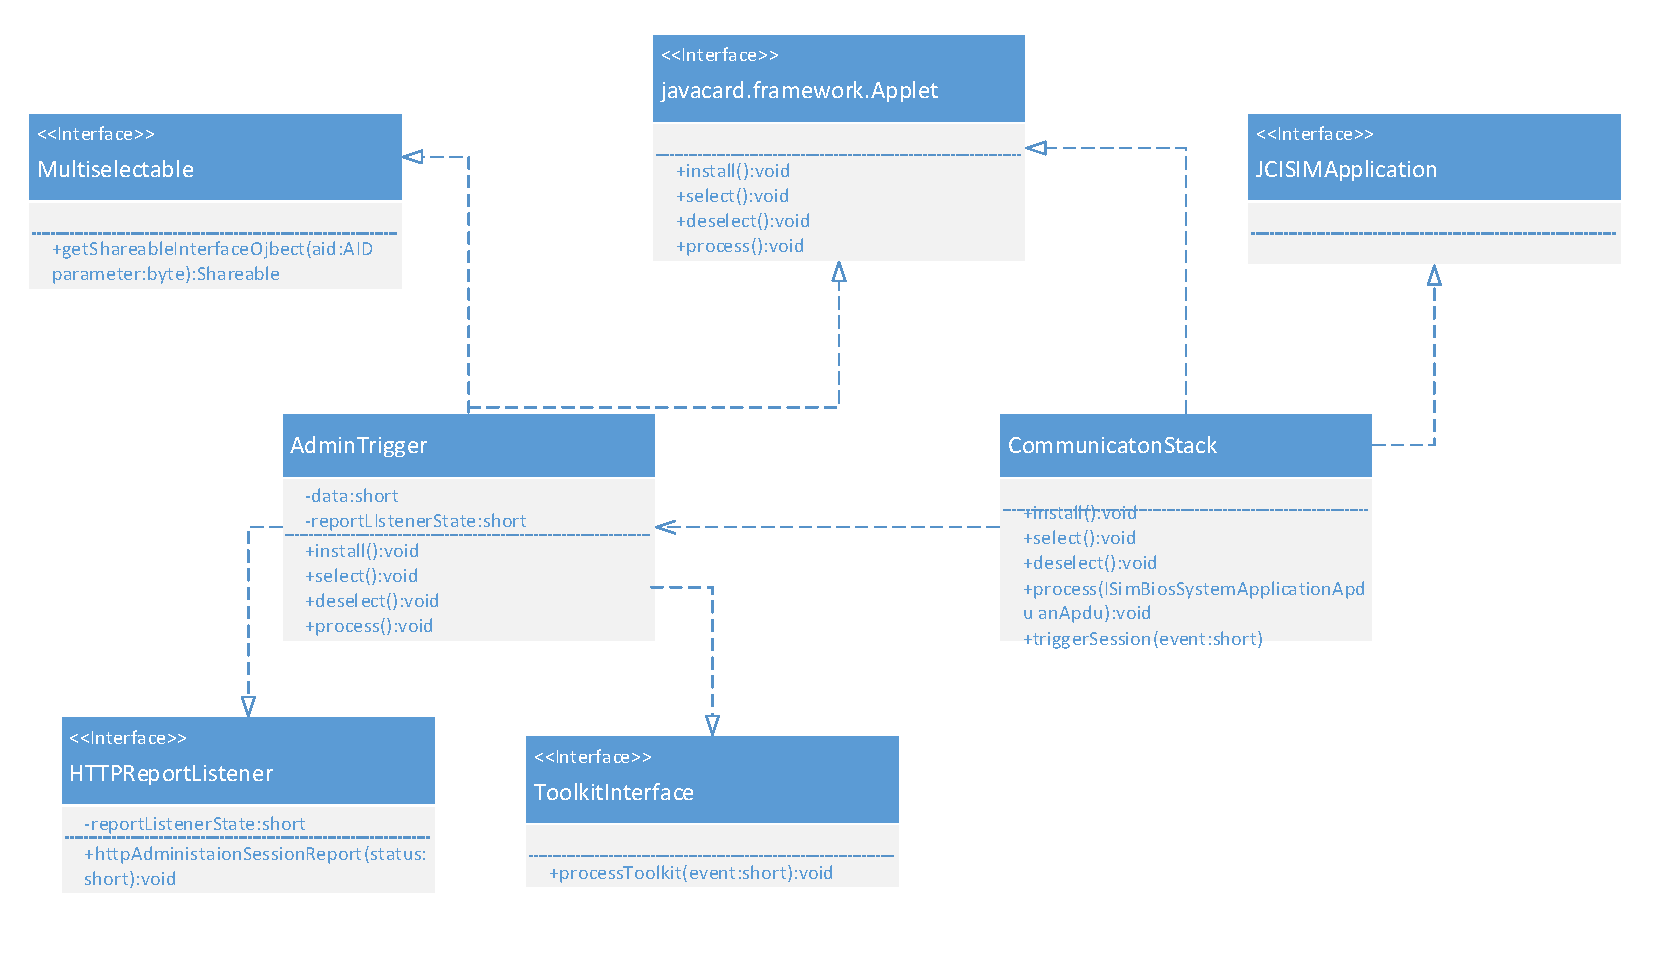
\includegraphics[width=1.0\textwidth]{class}
		\caption{Class Diagram}
	\label{fig:class}
\end{figure}

\subsubsection{Class CommunicationStack} \sloppy
As the main class of my Applet, \emph{communicationStack} extends \emph{UsimRemoteService} class provided by Morpho in order to be recognized as a system Applet, which is capable of performing remote application/file management behavior. Moreover this main class has implemented interface \emph{JCISIMApplication}, which defines mechanisms to handle remote APDUs.

Also PIN configuration is defined in this applet and described as below, 

\begin{Verbatim}[fontsize=\relsize{-1}]
    private static final byte PIN_TRY_LIMIT = (byte) 0x03;
    private static final byte PIN_MAX_SIZE = (byte) 0x08;
    private static final byte PIN_SIZE = (byte) 0x04;
\end{Verbatim}

System allows maximum three time wrong PIN input and PIN size is set from four bits to eight.
Following two core methods provided by \emph{communicationStack} is described.
\paragraph{Install Method}
\emph{install} method is used to register my applet in JCRE and create a CommunicationStack implementation.
\begin{Verbatim}[fontsize=\relsize{-1.5}, frame=lines,framesep=4mm, label=\fbox{\small\emph{doVerifyPIN Handler}}]
public static void install( byte[] bArray, short bOffset, byte bLength ) throws ISOException
\end{Verbatim}

\paragraph{process Method} \label{secDummy}
In this method, the received remote APDU command will be analyzed and upon on the encapsulated instruction filed, corresponding handler will be invoked based on the \emph{command data} included in the same command APDU. Following snippet defines how to get \emph{class} filed, \emph{instruction} filed , \emph{command data} and alternatively an normal \emph{APDU} object from a remote APDU object.


\begin{Verbatim}[frame=lines,framesep=4mm, label=\fbox{\small\emph{Remote APDU Operation}}]
byte claMasked = (byte)(anApdu.getCla() & (byte)0xF0);
byte ins = anApdu.getIns();
byte[] cmd = (byte[]) anApdu.getCommandData();	    
short cmdOffset = anApdu.getCommandDataOffset();
byte[] apdu = anApdu.getApdu(); //return APDU object if available
\end{Verbatim}

Based on the acknowledgment of \emph{claMasked} , \emph{ins} data and \emph{apdu} object, using below described switch statement, appropriate handler is invoked.

\begin{Verbatim}[frame=lines,framesep=4mm, label=\fbox{\small\emph{Switch Statement}}]
switch(ins)
	{
	case INS_VERIFYPIN:
		doVerifyPIN(apdu);
	case ....
	}
\end{Verbatim}
In case when \emph{ins} equals \emph{INS\_VERIFYPIN}, following \emph{doVerifyPIN} is invoked.

\begin{Verbatim}[fontsize=\relsize{-1}, frame=lines,framesep=4mm, label=\fbox{\small\emph{doVerifyPIN Handler}}]
private void doVerifyPIN(APDU apdu) {
	byte[] buffer = apdu.getBuffer();
	apdu.setIncomingAndReceive();			
	if(pin.getTriesRemaining() == (byte)0) {
		ISOException.throwIt(SW_PIN_BLOCKED);	
	....
	}
\end{Verbatim}
In total six handlers are designed:
\begin{itemize}
\item \emph{doVerifyPIN}. As already introduced, this handler performs the verify PIN operation. If wrong PIN input reaches 3 times before a successful verification, \emph{doVerfiyPIN} will block the PIN.
\item \emph{doResetPIN}.This handler in charge of reset PIN operation.
\item \emph{doUnlockPIN}. \emph{doUnlockPIN} operation will be and only be invoked by card issuer for the purpose of unlock blocked PIN.
\item \emph{doGetPublicKey}. This operation queries target public key from \emph{Public Key infrastructure} which is integrated in OTA server in my scenario.
\item \emph{doNotification}. After receiving command data, \emph{communicationStack} applet will invoke this handler in order to inform corresponding subscriber to fetch that command data. 
\item \emph{doAppendMsg}.  This handler configures the outgoing response remote APDU.
\end{itemize}
Except from statue words, if other information is expected to be transmitted back to the command APDU sender,  the return data can be appended at the end of existing response data buffer using following schema.

\begin{Verbatim}[fontsize=\relsize{-1}, frame=lines,framesep=4mm, label=\fbox{\small\emph{Editing Response Data}}]
byte[] result = {....};
short length = (short) result.length;
byte[] resBuff = anApdu.getResponseBuffer(); 
short resOffset = anApdu.getResponseBufferOffset();
Util.arrayCopyNonAtomic(result, (short)0, resBuff, (short)resOffset, (short)length);	    
anApdu.setStatusword(State_Word);
anApdu.appendResponse(resBuff,(short)resOffset, (short)length, true);
\end{Verbatim}

Byte array \emph{result} represents the appended data and \emph{resBuff} is the outgoing buffer. 

\subsubsection{Class SessionTrigger}
\emph{sessionTrigger} class extends \emph{HTTPReportListener} interface in order to receive notification upon completion of an session.
\emph{triggerSession} method as shown below provides core mechanism to create a communication session configured by input parameter \emph{byte[] data}.
\begin{Verbatim}[fontsize=\relsize{-2}, frame=lines,framesep=4mm, label=\fbox{\small\emph{Trigger Session}}]
public void triggerSession(byte[] data, short dataOffset, short dataLength )
 {
final short FAMILY_HTTP_ADMINISTRATION = (short) (GPSystem.FAMILY_HTTP_ADMINISTRATION << 8)
GlobalService globalService = GPSystem.getService(null, FAMILY_HTTP_ADMINISTRATION);
HTTPAdministration httpAdmin = (HTTPAdministration)globalService.getServiceInterface
(GPSystem.getRegistryEntry(null),FAMILY_HTTP_ADMINISTRATION, null, (short)0, (short)0);
httpAdmin.requestHTTPAdministrationSession(data, dataOffset, dataLength);
}
\end{Verbatim}

\section{Android Application}
In order to simulate and realize application level  OPC UA functionalities, I have designed the following Android Application.


\begin{figure}[!htb]
	\centering
	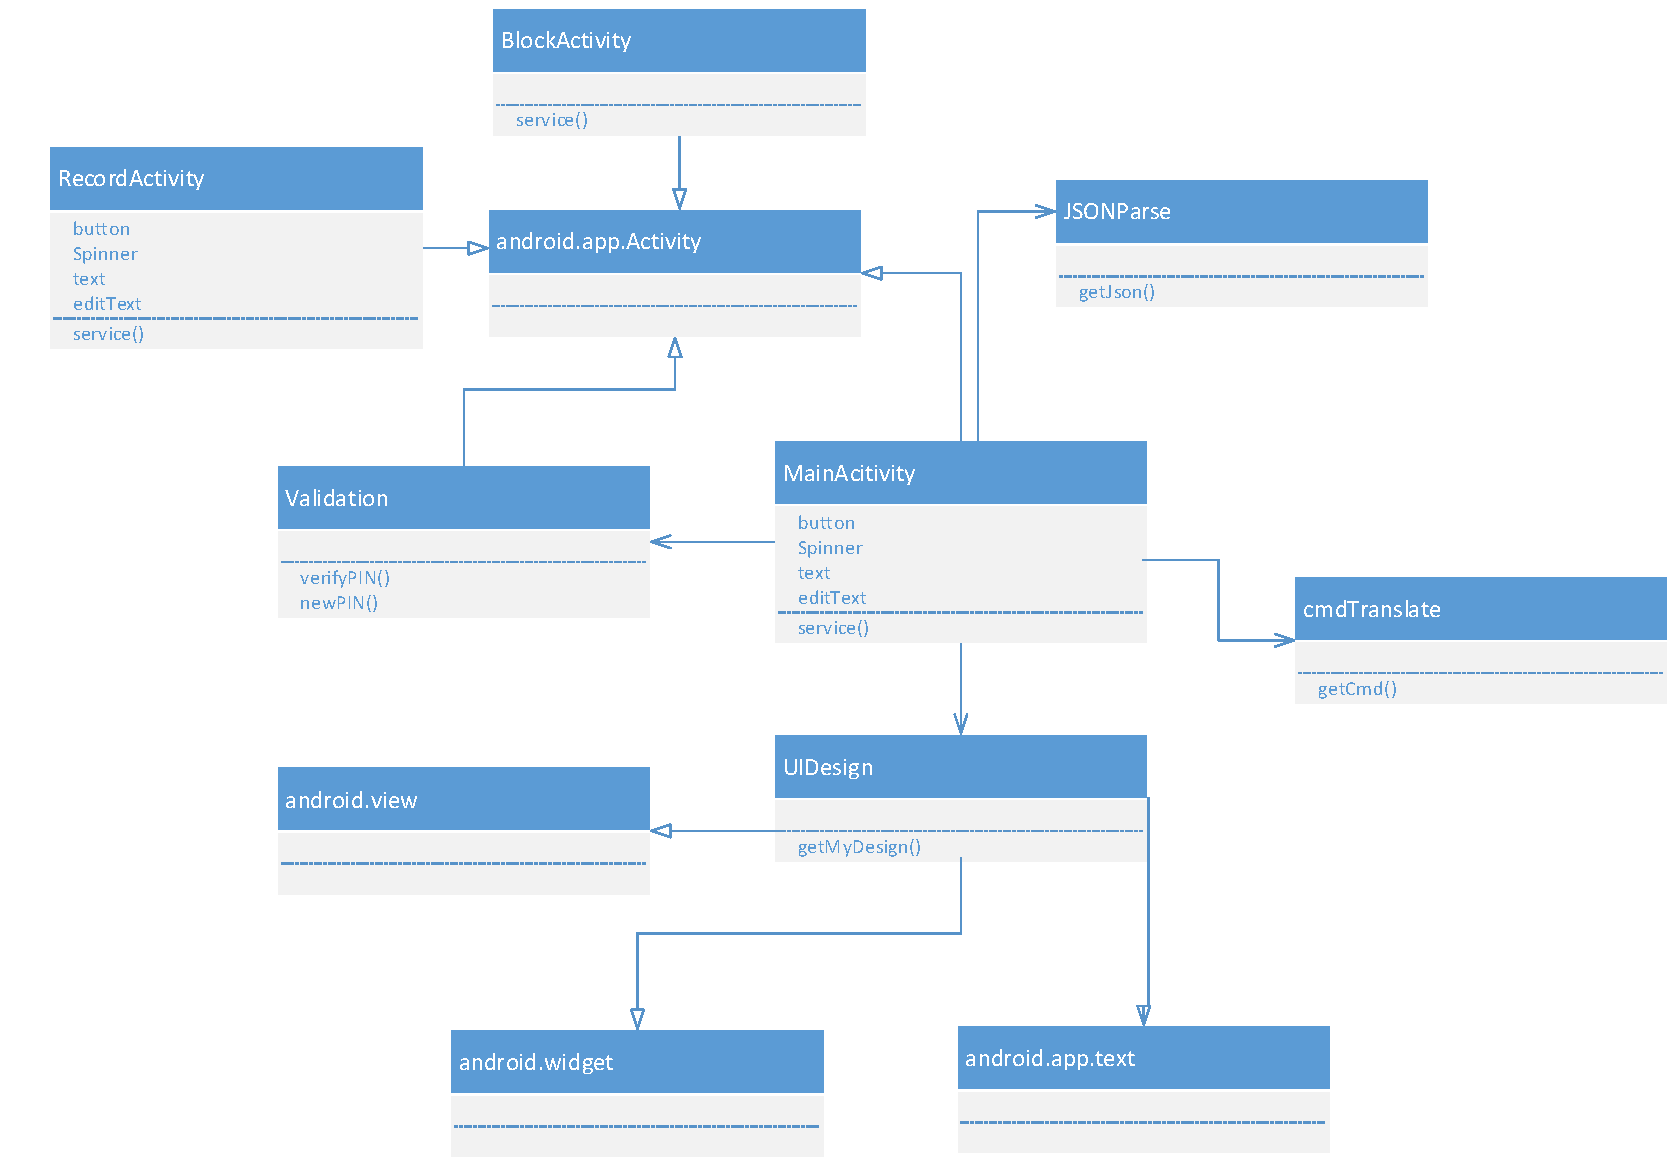
\includegraphics[width=1\textwidth]{android-class}
		\caption{Android Application Class Diagram}
	\label{fig:android-class}
\end{figure}

\subsection{Utility Classes}
The Application class diagram is shown in figure ~\ref{fig:android-class}. And in order to encapsulate commonly re-used functions, following utility classes are employed.
\begin{itemize}
\item \emph{CmdTranslate}. This class provide methods such as \emph{getCmd}, \emph{getCmdTlv} and \emph{byteArrayToHexString}, which are used to translate user commands into byte arrays based on rules defined in table~\ref{tlv}.
\item \emph{JSONParser}. With supports provided by \emph{org.apache.http} and \emph{org.json} packages, \emph{JSONParse} class offers mechanisms to generate Http POST and GET request. Moreover method \emph{makeHttpRequest} in this class returns a Json object including query result as well as return code.
\item \emph{UiDesign}. Based on package \emph{android.graphic} and \emph{android.text}, this class provides the approach to realize customized UIi layout. For instance, in method \emph{getStyle(String text, int begin, int end, String Farbe)}, the text between \emph{begin} and \emph{end} position is granted with a given color,  \emph{Farbe}. A concrete usage case is demonstrated in figure~\ref{fig:get-style}

\begin{figure}[!htbp]
	\centering
	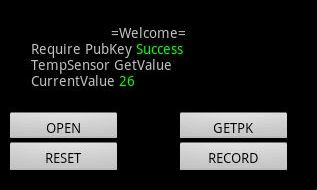
\includegraphics[width=0.55\textwidth]{get-style.jpg}
		\caption{Customized text color}
	\label{fig:get-style}
\end{figure}

\end{itemize} 
\subsection{Layout} \label{secLayout}
Under \emph{root$\backslash$res$\backslash$layout} directory, the \emph{xml} files that define layout frameworks of my application activities are presented. To be more specifically,
\begin{itemize}
\item \emph{welcome.xml}. The UI-layout of welcome screen is described, where user should input his password and username.
\item \emph{main.xml}, which defines the layout of main screen.
\item \emph{list\_item.xml} and \emph{record.xml}. Those two xml files together picture how to present historical record in a list arranged by modified data.
\item \emph{block.xml}. The PIN block screen is defined by \emph{block.xml}
\end{itemize}
The screen shots of my Android application will be presented in next chapter \emph{Implementation Test}.


\subsection{Activity Classes}
Activity class extends \emph{android.app.Activity} and implements interface \emph{SEService.CallBack} provided by Simalliance OpenMobileapi with whose help one activity is able to receive call-back from smart card. 
\subsubsection{Seek for Android}
Seek for Android is a smart card API that implements Simalliance OpenMobileAPI standards which grants Android application the ability to communicate with secure elements such as smart card. Package \emph{org.simalliance.openmobileapi} is the code realization of aforementioned specifications.

In order to connect with the smart card, the \emph{SEService} constructor must be generated, which provides the method \emph{getReaders} returning a list of available connected secure elements. If one \emph{reader} is selected, then with the help of \emph{openSession} method, one particular session will be created between the desire selected secure element and the application. At last this \emph{session} is capable of getting access to a logical channel on the connected secure element by applying \emph{openLogicalChannel} method with AID as input parameter. Following code snippet demonstrates the service and logical channel creation process\cite{open}.

\begin{Verbatim}[fontsize=\relsize{-1},frame=lines,framesep=4mm, label=\fbox{\small\emph{Service and logical channel Creation}}]
void performSelectOpt(SEService service) {
Reader[] readers = service.getReaders();
cardreader = readers[0].getName();
boolean isPresent = readers[0].isSecureElementPresent();
Session session = readers[0].openSession();
final byte[] hellosimcard = new byte[] {AID};
logicalChannel = session.openLogicalChannel(hellosimcard);
performOpenOpt(service);
}
\end{Verbatim}
After a successful creation of logical channel, one Android application is able to send command to and get response from a secure element using \emph{bytep[] result = logicalChannel.tramsmit(cmdApdu)}.
\subsubsection{Layout Adoption}
Activity class adopts the layout defined in~\ref{secLayout} during the activity creation phase.

\begin{Verbatim}[fontsize=\relsize{-1},frame=lines,framesep=4mm, label=\fbox{\small\emph{Layout Adoption}}]
public void onCreate(Bundle savedInstanceState) {
super.onCreate(savedInstanceState);
// set Layout
setContentView(R.layout.main);
\end{Verbatim}

\subsubsection{AsyncTask}
Since the \emph{HttpResponse} message could be delivered to \emph{activity} which sends the  corresponding \emph{HttpRequest} message with latency, therefore for the purpose of simplified UI thread operations, the interface \emph{AsyncTask} is employed in my application.

Following code snippet demonstrates class, that is used to perform sensor subscription value update operation. 
\begin{Verbatim}[fontsize=\relsize{-1},frame=lines,framesep=4mm, label=\fbox{\small\emph{AsyncTask HttpRequest}}]
class RecordUpdate extends AsyncTask<String, String, String> {
protected void onPreExecute() {}	
protected String doInBackground(String... params) {
runOnUiThread(new Runnable() {
public void run() {
...
JSONObject json = jsonParser.makeHttpRequest(url_update_record, "GET", params);
...
\end{Verbatim}
\subsubsection{Intent}
As already introduced in~\ref{secIntent}, intent builds data sharing system between activities. Following code segment describes how \emph{ValidationActivity} class perform page jump based on \emph{performVerifyOpt} result.
\begin{Verbatim}[fontsize=\relsize{-1},frame=lines,framesep=4mm, label=\fbox{\small\emph{Intent}}]
Intent intent = new Intent();           			  	
verifyResult = performVerifyOpt(scservice);
if (verifyResult == 1){
intent.setClass(Validation.this, MainActivity.class);  
startActivity(intent);  
finish(); }
if (verifyResult == 3){
intent.setClass(Validation.this, BlockActivity.class);  
startActivity(intent);  
finish(); }
\end{Verbatim}
\subsubsection{Activities Overview}
Following four activities together build my Android application.
\begin{itemize}
\item \emph{ValidationActivity}. Whose major task is to realize user authentication based on inputted user-name and password.
\item \emph{BlockActivity}. After three time wrong failed user identification, my application will invoke this \emph{BlockActivity} and accordingly block the PIN.
\item \emph{MainActivity}. This class realizes client functions defined in~\ref{secFunction}
\item \emph{RecordActivity}. With the help of \emph{RecordActivity}, user is capable of querying and viewing system historical data.
\end{itemize}

\subsubsection{AndroidManifest}
\emph{AndroidManifest} encapsulates all necessary information which is quired by Android OS. Such as composing components, access permissions and necessary libraries\cite{android_manifest}. In order to provide a secure application environment, in my \emph{AndroidManifest}, only the \emph{ValidationActivity} can be launched by Android system and always run as the initial task. Moreover, no \emph{intent-filters} are declared for my activities, which means they can only be started or visited by the explicit intent sent by \emph{ValidationActivity} as show below.
\begin{Verbatim}[fontsize=\relsize{-1},frame=lines,framesep=4mm, label=\fbox{\small\emph{AndroidManifest.xml}}]
<?xml version="1.0" encoding="utf-8"?>
<manifest xmlns:android="http://schemas.android.com/apk/res/android"
	android:versionCode="1"
	android:versionName="1.0" package="org.simalliance.openmobileapi.test">
 <application android:label="@string/app_name" android:debuggable="true">
  <activity android:name=".ValidationActivity"
 		android:label="@string/app_name">
	<intent-filter>
		<action android:name="android.intent.action.MAIN" />
		<category android:name="android.intent.category.LAUNCHER" />
	</intent-filter>
 </activity>
      
 <activity android:name=".MainActivity"
	android:label="@string/app_name"
	android:exported='false'>
 </activity>
....
 </application>
</manifest> 
\end{Verbatim}



\begin{figure}[!htb]
	\centering
	
\includegraphics[width=0.55\textwidth]{logo.png}
		\caption{Logo image used in web applications}
	\label{fig:logo}
\end{figure}

\section{Smart Home Web Server}
Smart Home web application are also designed for the purpose of testing my smart card applet, Android application as well as simulating Smart Home devices, especially the data information maintained by them. 
Apache 2.4.9 together with PhP of version 5.5.12 and MySQL database build my web applications.  
\begin{figure}[!htb]
	\centering
	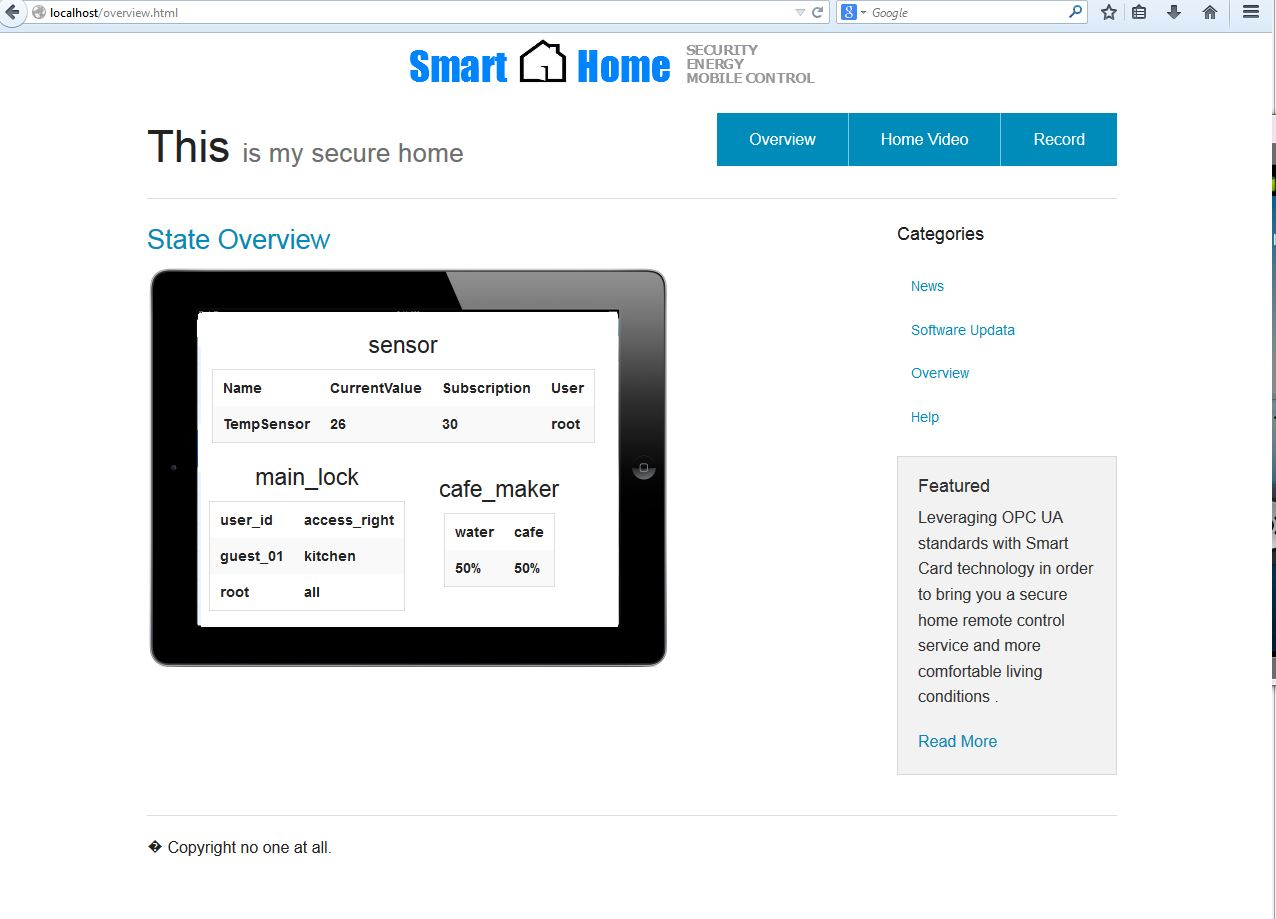
\includegraphics[width=1\textwidth]{Images/design/overview.jpg}
		\caption{Smart Home Web Overview}
	\label{fig:smart-home-frontpage}
\end{figure}

Figure ~\ref{fig:smart-home-frontpage} illustrates the web page that shows all three housing devices states. Each housing device has its own table in MySQL database. Moreover, user can navigate to other pages by clicking the blue tabs on top right of this page. For instance, by clicking \emph{Record} button, user is able to bowser historical record of each home device. 
Detailed design process has limited relation with the subject of this thesis, therefor will not be presented.